\subsection{Architekturmuster (Patterns)}

\begin{concept}{Architekturmuster Übersicht}\\
Grundlegende Architekturmuster für verteilte Systeme:
\begin{itemize}
    \item \textbf{Layered Pattern:} Schichtenarchitektur
    \item \textbf{Client-Server Pattern:} Verteilte Dienste
    \item \textbf{Master-Slave Pattern:} Verteilte Verarbeitung
    \item \textbf{Pipe-Filter Pattern:} Datenstromverarbeitung
    \item \textbf{Broker Pattern:} Vermittler zwischen Endpunkten
    \item \textbf{Event-Bus Pattern:} Nachrichtenverteilung
    \item \textbf{MVC Pattern:} Trennung von Daten und Darstellung
\end{itemize}
\end{concept}

\begin{example2}{Layered Pattern}\\
\textbf{Struktur:}
\begin{lstlisting}[language=Java, style=basesmol]
// Presentation Layer
public class CustomerUI {
    private CustomerService service;
    public void showCustomerDetails(int id) {
        Customer customer = service.getCustomer(id);
        // display logic
    }
}

// Business Layer
public class CustomerService {
    private CustomerRepository repository;
    public Customer getCustomer(int id) {
        return repository.findById(id);
    }
}

// Data Layer
public class CustomerRepository {
    public Customer findById(int id) {
        // database access
        return customer;
    }
}
\end{lstlisting}

\textbf{Vorteile:}
\begin{itemize}
    \item Klare Trennung der Verantwortlichkeiten
    \item Austauschbarkeit einzelner Schichten
    \item Einfachere Wartung und Tests
\end{itemize}
\end{example2}

\begin{KR}{Clean Architecture}\\
Prinzipien nach Robert C. Martin:

\begin{itemize}
    \item \textbf{Unabhängigkeit von Frameworks}
    \begin{itemize}
        \item Framework als Tool, nicht als Einschränkung
        \item Geschäftslogik unabhängig von UI/DB
    \end{itemize}
    
    \item \textbf{Testbarkeit}
    \begin{itemize}
        \item Business Rules ohne externe Systeme testbar
        \item Keine DB/UI für Tests notwendig
    \end{itemize}
    
    \item \textbf{Unabhängigkeit von UI}
    \begin{itemize}
        \item UI austauschbar ohne Business Logic Änderung
        \item Web, Desktop, Mobile möglich
    \end{itemize}
    
    \item \textbf{Unabhängigkeit von Datenbank}
    \begin{itemize}
        \item DB-System austauschbar
        \item Business Rules unabhängig von Datenpersistenz
    \end{itemize}
\end{itemize}

\textbf{Schichten von außen nach innen:}
\begin{enumerate}
    \item Frameworks \& Drivers (UI, DB, External Interfaces)
    \item Interface Adapters (Controllers, Presenters)
    \item Application Business Rules (Use Cases)
    \item Enterprise Business Rules (Entities)
\end{enumerate}
\end{KR}

\begin{example2}{Clean Architecture Implementation}\\
\textbf{Strukturbeispiel für einen Online-Shop:}

\begin{lstlisting}[language=Java, style=basesmol]
// Enterprise Business Rules (Entities)
public class Order {
    private List<OrderItem> items;
    private OrderStatus status;
    
    public Money calculateTotal() {
        return items.stream()
                   .map(OrderItem::getSubtotal)
                   .reduce(Money.ZERO, Money::add);
    }
}

// Application Business Rules (Use Cases)
public class CreateOrderUseCase {
    private OrderRepository repository;
    private PaymentGateway paymentGateway;
    
    public OrderId execute(CreateOrderCommand command) {
        Order order = new Order(command.getItems());
        PaymentResult result = paymentGateway.process(
            order.calculateTotal());
        if (result.isSuccessful()) {
            return repository.save(order);
        }
        throw new PaymentFailedException();
    }
}

// Interface Adapters
public class OrderController {
    private CreateOrderUseCase createOrderUseCase;
    
    public OrderResponse createOrder(OrderRequest request) {
        CreateOrderCommand command = mapToCommand(request);
        OrderId id = createOrderUseCase.execute(command);
        return new OrderResponse(id);
    }
}
\end{lstlisting}
\end{example2}

\begin{concept}{Microservices Architektur}\\
\textbf{Grundprinzipien:}
\begin{itemize}
    \item Unabhängig deploybare Services
    \item Lose Kopplung
    \item Eigene Datenhaltung pro Service
    \item REST/Message-basierte Kommunikation
\end{itemize}

\textbf{Vorteile:}
\begin{itemize}
    \item Bessere Skalierbarkeit
    \item Unabhängige Entwicklung
    \item Technologiefreiheit
    \item Robustheit
\end{itemize}

\textbf{Herausforderungen:}
\begin{itemize}
    \item Verteilte Transaktionen
    \item Service Discovery
    \item Datenkonvergenz
    \item Monitoring
\end{itemize}
\end{concept}

\begin{example2}{Microservice Design}\\
\textbf{Service für Benutzerprofile:}

\begin{lstlisting}[language=Java, style=basesmol]
@RestController
@RequestMapping("/api/users")
public class UserProfileController {
    private final UserService userService;
    
    @GetMapping("/{id}")
    public UserProfileDTO getProfile(@PathVariable String id) {
        UserProfile profile = userService.findById(id);
        return UserProfileDTO.from(profile);
    }
    
    @PutMapping("/{id}")
    public ResponseEntity<Void> updateProfile(
            @PathVariable String id, 
            @RequestBody UpdateProfileCommand command) {
        userService.updateProfile(id, command);
        return ResponseEntity.ok().build();
    }
}

// Event fuer andere Services
public class UserProfileUpdatedEvent {
    private final String userId;
    private final String newEmail;
    private final LocalDateTime timestamp;
    
    // Konstruktor und Getter
}
\end{lstlisting}
\end{example2}

\begin{KR}{Microservices Design Prinzipien}\\
\textbf{1. Service Boundaries}
\begin{itemize}
    \item Nach Business Capabilities trennen
    \item Bounded Context (DDD) beachten
    \item Datenhoheit festlegen
\end{itemize}

\textbf{2. Service Kommunikation}
\begin{itemize}
    \item Synchron vs. Asynchron
    \item Event-Driven Design
    \item API Gateway Pattern
\end{itemize}

\textbf{3. Datenmanagement}
\begin{itemize}
    \item Database per Service
    \item Event Sourcing
    \item CQRS Pattern
\end{itemize}

\textbf{4. Resilience}
\begin{itemize}
    \item Circuit Breaker
    \item Bulkhead Pattern
    \item Fallback Mechanismen
\end{itemize}
\end{KR}

\subsection{Design Patterns in der Architektur}

\begin{concept}{Model-View-Controller (MVC)}\\
Trennt Anwendung in drei Hauptkomponenten:
\begin{itemize}
    \item \textbf{Model:} Geschäftslogik und Daten
    \item \textbf{View:} Darstellung der Daten
    \item \textbf{Controller:} Steuerung und Koordination
\end{itemize}

\begin{lstlisting}[language=Java, style=basesmol]
// Model
public class CustomerModel {
    private String name;
    private List<Order> orders;
    
    public void addOrder(Order order) {
        orders.add(order);
        notifyViews();
    }
}

// View
public class CustomerView {
    private CustomerModel model;
    
    public void displayCustomerInfo() {
        System.out.println("Customer: " + model.getName());
        System.out.println("Orders: " + model.getOrders().size());
    }
}

// Controller
public class CustomerController {
    private CustomerModel model;
    private CustomerView view;
    
    public void createOrder(OrderData data) {
        Order order = new Order(data);
        model.addOrder(order);
        view.displayCustomerInfo();
    }
}
\end{lstlisting}
\end{concept}

\begin{concept}{Event-Driven Architecture (EDA)}\\
Basiert auf der Produktion, Erkennung und Reaktion auf Events:

\textbf{Komponenten:}
\begin{itemize}
    \item Event Producer
    \item Event Channel
    \item Event Consumer
    \item Event Processor
\end{itemize}

\begin{lstlisting}[language=Java, style=basesmol]
// Event Definition
public class OrderCreatedEvent {
    private final String orderId;
    private final LocalDateTime timestamp;
    private final BigDecimal totalAmount;
}

// Event Producer
public class OrderService {
    private EventBus eventBus;
    
    public void createOrder(OrderData data) {
        Order order = orderRepository.save(data);
        OrderCreatedEvent event = new OrderCreatedEvent(
            order.getId(),
            LocalDateTime.now(),
            order.getTotalAmount()
        );
        eventBus.publish(event);
    }
}

// Event Consumer
@EventListener
public class InvoiceGenerator {
    public void handleOrderCreated(OrderCreatedEvent event) {
        generateInvoice(event.getOrderId());
    }
}
\end{lstlisting}
\end{concept}

\begin{KR}{Architektur-Dokumentation}\\
\textbf{1. Überblick}
\begin{itemize}
    \item Systemkontext
    \item Hauptkomponenten
    \item Technologie-Stack
\end{itemize}

\textbf{2. Architektur-Entscheidungen}
\begin{itemize}
    \item Begründungen
    \item Alternativen
    \item Trade-offs
\end{itemize}

\textbf{3. Technische Konzepte}
\begin{itemize}
    \item Persistenz
    \item Sicherheit
    \item Integration
    \item Deployment
\end{itemize}

\textbf{4. Qualitätsszenarien}
\begin{itemize}
    \item Performance
    \item Skalierbarkeit
    \item Verfügbarkeit
    \item Wartbarkeit
\end{itemize}
\end{KR}

\begin{example2}{Architektur-Dokumentation: REST API}\\
\textbf{API-Design und Dokumentation:}

\begin{lstlisting}[language=Java, style=basesmol]
@RestController
@RequestMapping("/api/v1/orders")
public class OrderController {
    
    @GetMapping("/{id}")
    @Operation(summary = "Get order by ID",
              description = "Returns detailed order information")
    @ApiResponses({
        @ApiResponse(responseCode = "200", 
                    description = "Order found"),
        @ApiResponse(responseCode = "404", 
                    description = "Order not found")
    })
    public OrderDTO getOrder(@PathVariable String id) {
        return orderService.findById(id)
                          .map(OrderDTO::from)
                          .orElseThrow(OrderNotFoundException::new);
    }
}
\end{lstlisting}

\textbf{Qualitätsszenarien:}
\begin{itemize}
    \item Response Time < 200ms (95. Perzentil)
    \item Verfügbarkeit 99.9%
    \item Maximal 1000 req/s pro Instance
    \item Automatische Skalierung ab 70% CPU
\end{itemize}
\end{example2}


\section{Softwarearchitektur und Design old}

\begin{concept}{Überblick Softwareentwicklung}\\
Die Entwicklung von Software erfolgt in verschiedenen Ebenen:
\begin{itemize}
    \item Business Analyse (Domänenmodell, Requirements)
    \item Architektur (Logische Struktur)
    \item Entwicklung (Konkrete Umsetzung)
\end{itemize}
%todo: better resolution image
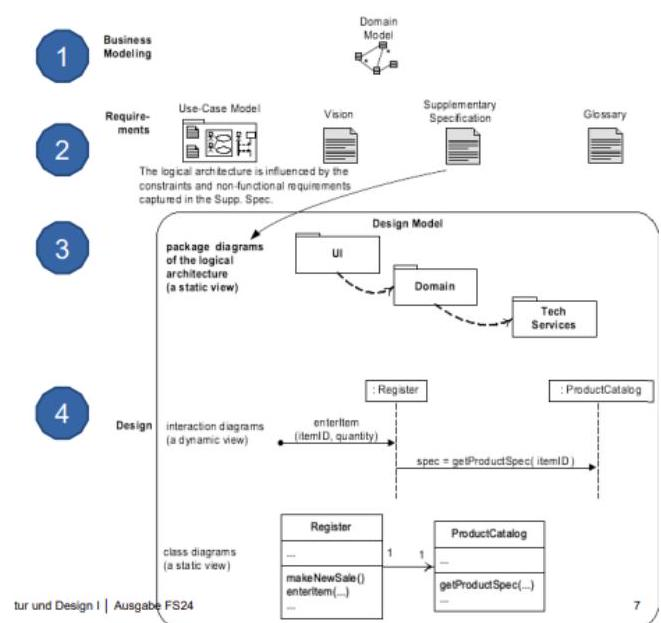
\includegraphics[width=\linewidth]{images/2024_12_29_0d1d7b5551ea1b4b41bdg-07(2)}
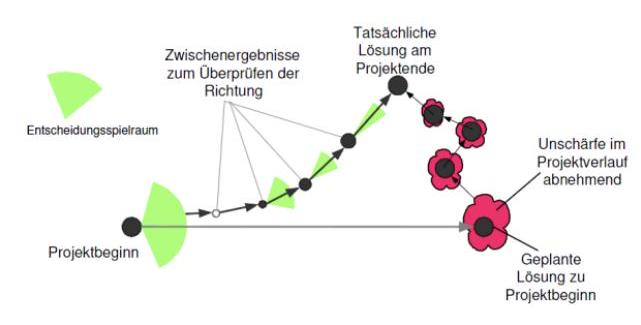
\includegraphics[width=\linewidth]{images/2024_12_29_0d1d7b5551ea1b4b41bdg-08(1)}
\end{concept}

\columnbreak

\subsubsection{Architektur}

\begin{definition}{Softwarearchitektur}\\
Die Architektur definiert:
\begin{itemize}
    \item Grundlegende Strukturen und Komponenten
    \item Heutige und zukünftige Anforderungen
    \item Weiterentwicklungsmöglichkeiten
    \item Beziehungen zur Umgebung
\end{itemize}
\end{definition}

\begin{concept}{Architekturanalyse}\\
Die Analyse erfolgt iterativ mit den Anforderungen:
\begin{itemize}
    \item Analyse funktionaler und nicht-funktionaler Anforderungen
    \item Abstimmung mit Stakeholdern
    \item Kontinuierliche Weiterentwicklung
\end{itemize}
%todo: better resolution image
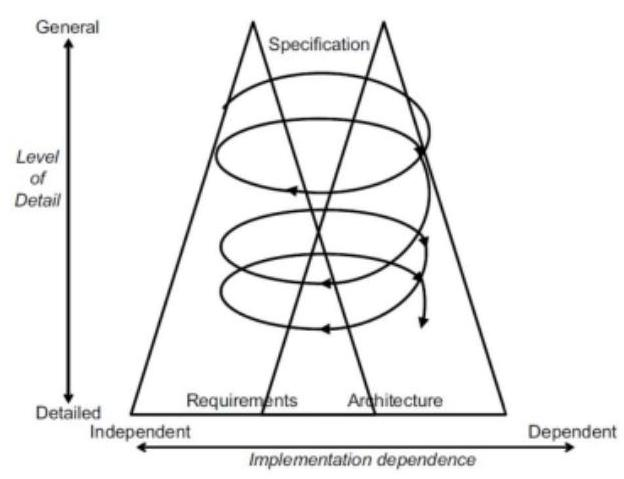
\includegraphics[width=0.9\linewidth]{images/2024_12_29_0d1d7b5551ea1b4b41bdg-08}
\end{concept}



\begin{theorem}{ISO 25010 vs FURPS+}\\
\textbf{ISO 25010:}
\begin{itemize}
    \item Hierarchische Struktur für nicht-funktionale Anforderungen
    \item Definierte Hauptcharakteristiken und Subcharakteristiken
    \item Messbare Metriken für jede Anforderung
    \item Präzise Formulierung und Verifikation
\end{itemize}

\textbf{FURPS+:}
\begin{itemize}
    \item Functionality (Funktionalität)
    \item Usability (Benutzbarkeit)
    \item Reliability (Zuverlässigkeit)
    \item Performance (Leistung)
    \item Supportability (Wartbarkeit)
    \item + (Implementation, Interface, Operations, Packaging, Legal)
\end{itemize}
\end{theorem}

\begin{concept}{Modulkonzept}\\
Ein Modul (Baustein, Komponente) wird bewertet nach:
\begin{itemize}
    \item \textbf{Kohäsion:} Innerer Zusammenhang
    \item \textbf{Kopplung:} Externe Abhängigkeiten
\end{itemize}

\textbf{Eigenschaften:}
\begin{itemize}
    \item Autarkes Teilsystem
    \item Minimale externe Schnittstellen
    \item Enthält alle benötigten Funktionen/Daten
    \item Verschiedene Formen: Paket, Library, Service
\end{itemize}
\end{concept}

\begin{concept}{Architektursichten}\\
Das N+1 View Model beschreibt verschiedene Perspektiven:\\
%todo: better resolution image
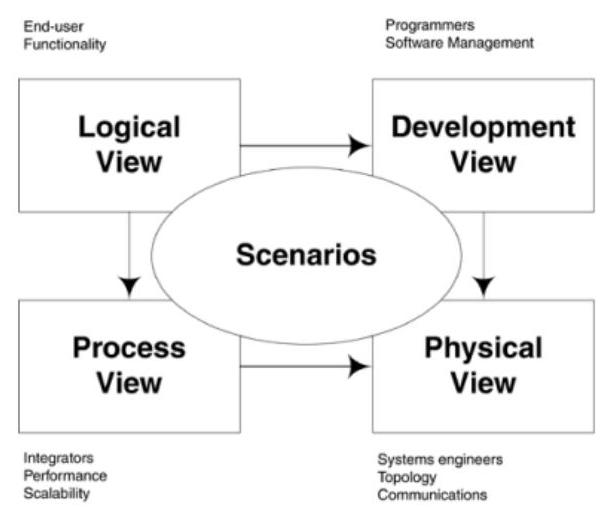
\includegraphics[width=0.9\linewidth]{images/2024_12_29_0d1d7b5551ea1b4b41bdg-09}
\end{concept}

\begin{KR}{Architekturentwurf}\\
\textbf{Schritte:}
\begin{enumerate}
    \item Anforderungen analysieren
    \item Architekturstil wählen
    \item Module identifizieren
    \item Schnittstellen definieren
    \item Mit Stakeholdern abstimmen
\end{enumerate}

\textbf{Qualitätskriterien:}
\begin{itemize}
    \item Änderbarkeit
    \item Wartbarkeit
    \item Erweiterbarkeit
    \item Testbarkeit
\end{itemize}
\end{KR}

\begin{example2}{Architekturentwurf}\\
\textbf{Aufgabe:} Entwerfen Sie die grundlegende Architektur für ein Online-Banking-System.

\textbf{Lösung:}
\begin{itemize}
    \item \textbf{Anforderungsanalyse:}
    \begin{itemize}
        \item Sicherheit (ISO 25010)
        \item Performance (FURPS+)
        \item Skalierbarkeit
    \end{itemize}
    
    \item \textbf{Architekturentscheidungen:}
    \begin{itemize}
        \item Mehrschichtige Architektur
        \item Microservices für Skalierbarkeit
        \item Sicherheitsschicht
    \end{itemize}
    
    \item \textbf{Module:}
    \begin{itemize}
        \item Authentifizierung
        \item Transaktionen
        \item Kontoführung
    \end{itemize}
\end{itemize}
\end{example2}

\begin{KR}{Architekturentscheidungen treffen}\\
Systematischer Ansatz für Architekturentscheidungen:
\begin{enumerate}
    \item \textbf{Anforderungen analysieren}
    \begin{itemize}
        \item Funktionale Anforderungen gruppieren
        \item Nicht-funktionale Anforderungen priorisieren
        \item Randbedingungen identifizieren
    \end{itemize}
    
    \item \textbf{Einflussfaktoren bewerten}
    \begin{itemize}
        \item Technische Faktoren
        \item Organisatorische Faktoren
        \item Wirtschaftliche Faktoren
    \end{itemize}
    
    \item \textbf{Alternativen evaluieren}
    \begin{itemize}
        \item Vor- und Nachteile abwägen
        \item Proof of Concepts durchführen
        \item Risiken analysieren
    \end{itemize}
    
    \item \textbf{Entscheidung dokumentieren}
    \begin{itemize}
        \item Begründung festhalten
        \item Verworfene Alternativen dokumentieren
        \item Annahmen dokumentieren
    \end{itemize}
\end{enumerate}
\end{KR}

\begin{example2}{Typische Prüfungsaufgabe: Architekturanalyse}\\
\textbf{Aufgabenstellung:}
Analysieren Sie folgende Anforderungen und leiten Sie architektonische Konsequenzen ab:
\begin{itemize}
    \item System muss 24/7 verfügbar sein
    \item 10.000 gleichzeitige Benutzer
    \item Reaktionszeit unter 1 Sekunde
    \item Jährliche Wartungsfenster maximal 4 Stunden
\end{itemize}

\textbf{Lösung:}
\begin{itemize}
    \item \textbf{Architekturentscheidungen:}
    \begin{itemize}
        \item Verteilte Architektur für Hochverfügbarkeit
        \item Load Balancing für gleichzeitige Benutzer
        \item Caching-Strategien für Performanz
        \item Blue-Green Deployment für Wartung
    \end{itemize}
    
    \item \textbf{Begründungen:}
    \begin{itemize}
        \item Verteilung minimiert Single Points of Failure
        \item Load Balancer verteilt Last gleichmäßig
        \item Caching reduziert Datenbankzugriffe
        \item Blue-Green erlaubt Updates ohne Downtime
    \end{itemize}
\end{itemize}
\end{example2}



\begin{KR}{Architektur-Review durchführen}\\
\textbf{Vorgehen:}
\begin{enumerate}
    \item \textbf{Vorbereitung}
    \begin{itemize}
        \item Architektur-Dokumentation zusammenstellen
        \item Review-Team zusammenstellen
        \item Checklisten vorbereiten
    \end{itemize}
    
    \item \textbf{Durchführung}
    \begin{itemize}
        \item Architektur vorstellen
        \item Anforderungen prüfen
        \item Entscheidungen hinterfragen
        \item Risiken identifizieren
    \end{itemize}
    
    \item \textbf{Nachbereitung}
    \begin{itemize}
        \item Findings dokumentieren
        \item Maßnahmen definieren
        \item Follow-up planen
    \end{itemize}
\end{enumerate}

\textbf{Prüfkriterien:}
\begin{itemize}
    \item Anforderungserfüllung
    \item Technische Machbarkeit
    \item Zukunftssicherheit
    \item Best Practices
\end{itemize}
\end{KR}

\begin{example2}{Typische Prüfungsaufgabe: Architektur-Review}\\
    %todo: add example
\end{example2}


\subsubsection{UML-Modellierung}

\begin{KR}{Statische vs. Dynamische Modelle}\\
\textbf{Statische Modelle (Struktur):}
\begin{itemize}
    \item UML-Klassendiagramm
    \item Fokus auf Pakete, Klassen, Attribute
    \item Keine Methodenimplementierung
\end{itemize}

\textbf{Dynamische Modelle (Verhalten):}
\begin{itemize}
    \item UML-Interaktionsdiagramme
    \item Fokus auf Logik und Verhalten
    \item Implementierung der Methoden
\end{itemize}
\end{KR}

\begin{definition}{UML-Diagrammtypen}\\
    %todo: add missing diagram types
\textbf{1. Klassendiagramm:}
\begin{itemize}
    \item Klassen und aktive Klassen
    \item Attribute und Operationen
    \item Sichtbarkeiten und Beziehungen
    \item Interfaces und Realisierungen
\end{itemize}

\textbf{2. Sequenzdiagramm:}
\begin{itemize}
    \item Lebenslinien und Nachrichten
    \item Synchrone/Asynchrone Kommunikation
    \item Aktivierung und Deaktivierung
    \item Alternative Abläufe
\end{itemize}

\textbf{3. Zustandsdiagramm:}
\begin{itemize}
    \item Zustände und Übergänge
    \item Start- und Endzustände
    \item Composite States
    \item Historie und Parallelität
\end{itemize}

\textbf{4. Aktivitätsdiagramm:}
\begin{itemize}
    \item Aktionen und Aktivitäten
    \item Kontroll- und Datenflüsse
    \item Verzweigungen und Zusammenführungen
    \item Partitionen (Swimlanes)
\end{itemize}
\end{definition}

\begin{definition}{UML-Paketdiagramm:}
\begin{itemize}
    \item Definition von Teilsystemen
    \item Gruppierung von Elementen
    \item Abhängigkeiten zwischen Paketen
\end{itemize}
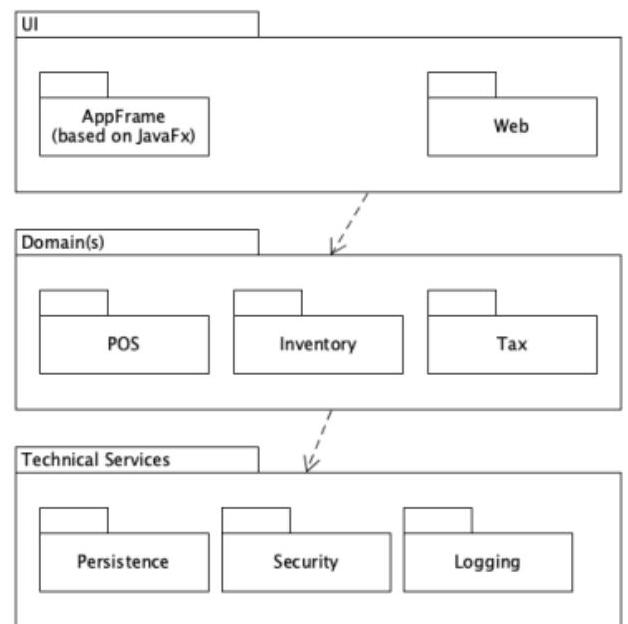
\includegraphics[width=0.9\linewidth]{images/2024_12_29_0d1d7b5551ea1b4b41bdg-09(1)}
\end{definition}

\begin{KR}{UML Diagrammauswahl}\\
Entscheidungshilfe für die Wahl des UML-Diagrammtyps:

\textbf{1. Strukturbeschreibung benötigt:}
\begin{itemize}
    \item Klassendiagramm für Typen und Beziehungen
    \item Paketdiagramm für Modularisierung
    \item Komponentendiagramm für Bausteinsicht
    \item Verteilungsdiagramm für Deployment
\end{itemize}

\textbf{2. Verhaltensbeschreibung benötigt:}
\begin{itemize}
    \item Sequenzdiagramm für Interaktionsabläufe
    \item Aktivitätsdiagramm für Workflows
    \item Zustandsdiagramm für Objektlebenszyklen
    \item Kommunikationsdiagramm für Objektkollaborationen
\end{itemize}

\textbf{3. Abstraktionsebene wählen:}
\begin{itemize}
    \item Analyse: Konzeptuelle Diagramme
    \item Design: Detaillierte Spezifikation
    \item Implementation: Codenahes Design
\end{itemize}
\end{KR}

\begin{concept}{Responsibility Driven Design (RDD)}\\
Design basierend auf Verantwortlichkeiten:
\begin{itemize}
    \item Klassenentwurf nach Rollen
    \item Kollaborationsbeziehungen
    \item Implementierung durch Attribute/Methoden
    \item Anwendbar auf allen Ebenen
\end{itemize}
\end{concept}

\begin{example2}{Prüfungsaufgabe: UML-Modellierung}
\textbf{Aufgabe:} 
Modellieren Sie für ein Bibliothekssystem die Ausleihe eines Buches mit:
\begin{itemize}
    \item Klassendiagramm der beteiligten Klassen
    \item Sequenzdiagramm des Ausleihvorgangs
    \item Zustandsdiagramm für ein Buchexemplar
\end{itemize}

\textbf{Bewertungskriterien:}
\begin{itemize}
    \item Korrekte UML-Notation
    \item Vollständigkeit der Modellierung
    \item Konsistenz zwischen Diagrammen
    \item Angemessener Detaillierungsgrad
\end{itemize}
%todo: add uml diagram
\end{example2}

\begin{theorem}{GRASP Prinzipien}\\
General Responsibility Assignment Software Patterns:
\begin{itemize}
    \item \textbf{Information Expert:} Verantwortung basierend auf Information
    \item \textbf{Creator:} Objekterstellung bei starker Beziehung
    \item \textbf{Controller:} Zentrale Steuerungslogik
    \item \textbf{Low Coupling:} Minimale Abhängigkeiten
    \item \textbf{High Cohesion:} Starker innerer Zusammenhang
    \item \textbf{Polymorphism:} Flexibilität durch Schnittstellen
    \item \textbf{Pure Fabrication:} Künstliche Klassen für besseres Design
    \item \textbf{Indirection:} Vermittler für Flexibilität
    \item \textbf{Protected Variations:} Kapselung von Änderungen
\end{itemize}
\end{theorem}

\begin{example2}{GRASP Anwendung}\\
\textbf{Szenario:} Online-Shop Warenkorb-Funktionalität

\textbf{GRASP-Prinzipien angewandt:}
\begin{itemize}
    \item \textbf{Information Expert:}
    \begin{itemize}
        \item Warenkorb kennt seine Positionen
        \item Berechnet selbst Gesamtsumme
    \end{itemize}
    
    \item \textbf{Creator:}
    \begin{itemize}
        \item Warenkorb erstellt Warenkorbpositionen
        \item Bestellung erstellt aus Warenkorb
    \end{itemize}
    
    \item \textbf{Controller:}
    \begin{itemize}
        \item ShoppingController koordiniert UI und Domain
        \item Keine Geschäftslogik im Controller
    \end{itemize}
    
    \item \textbf{Low Coupling:}
    \begin{itemize}
        \item UI kennt nur Controller
        \item Domain unabhängig von UI
    \end{itemize}
\end{itemize}
\end{example2}



